\documentclass[../../Cours_M1.tex]{subfiles}

\newcommand{\nomTD}{TP4: Modulation et démodulation de fréquence}
\renewcommand{\nomentete}{UE431 - \nomTD}
\renewcommand{\auteur}{Aymeric Arnould, Tom Colinot}


\renewcommand{\thesection}{\Roman{section}}
\renewcommand{\thesubsection}{\arabic{subsection}}

\begin{document}

\titre{\nomTD}

\begin{center}
\begin{Large}
A. Préparation
\end{Large}
\end{center}

\section{Modulation de fréquence}

\subsection*{Définitions}
On chercher à transmettre un signal informatif sinusoïdal \[s_{inf}(t) = S_m\cos(2\pi Ft)\]

Le signal modulé est $s(t)=S_p\cos(\Phi(t))$, où $\Phi(t)$ contient l'information à transmettre :
\[ \Phi(t) = 2\pi f_0 t + \int_0^t 2\pi K_f s_{inf}(u)du \]

\subsection*{Propriétés d'une onde modulée en fréquence}
\begin{itemize}\setlength{\itemsep}{10mm}
\item Avec les notations précédentes, on a 
\begin{align*}
s(t) & = S_p\cos(2\pi f_0 t + \int_0^t 2\pi K_f s_{inf}(u)du) \\
& = S_p\cos(2\pi f_0t + 2\pi K_f S_m \frac{1}{2\pi F} \sin(2\pi F t) \\
s(t) & = S_p\cos(2\pi f_0 t + \beta \sin(2\pi F t) \quad \avec \beta = \frac{\Delta f}{F} \et \Delta f = K_fS_m
\end{align*}

\item Grâce à l'identité de Bessel, on peut écrire
\[s(t) = S_p \sum_{n=-\infty}^{n=+\infty} J_n(\beta)\cos(2\pi (f_0+nF)t)\]
Sachant que $|J_n(beta)|=|J_{-n}(\beta)|$, le spectre de $s(t)$ sera constitué de raies symétriques autour d'une raie à $f_0$. Théoriquement, ce spectre a un support spectral infini.

\begin{figure}[h!]
\centering
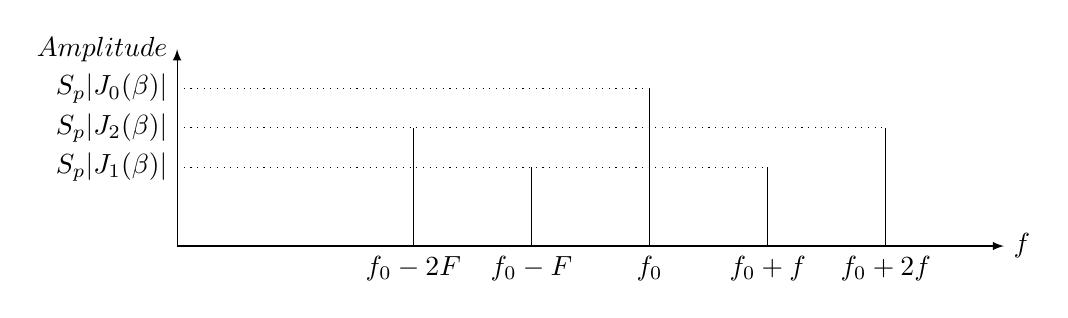
\begin{tikzpicture}[xscale=1.5]
\draw [>=latex,->] (0,0) -- (7,0) node[right]{$f$} ;
\draw [>=latex,->] (0,0) -- (0,2.5) node[left]{$Amplitude$};
\draw (4,0)node[below]{$f_0$} -- (4,2);
\draw (3,0)node[below]{$f_0-F$} -- (3,1);
\draw (5,0)node[below]{$f_0+f$} -- (5,1);
\draw (2,0)node[below]{$f_0-2F$} -- (2,1.5);
\draw (6,0)node[below]{$f_0+2f$} -- (6,1.5);
\draw [dotted] (0,2) node[left]{$S_p|J_0(\beta)|$} -- (4,2);
\draw [dotted] (0,1) node[left]{$S_p|J_1(\beta)|$} -- (5,1);
\draw [dotted] (0,1.5) node[left]{$S_p|J_2(\beta)|$} -- (6,1.5);
\end{tikzpicture}
\caption{Allure du spectre de $s(t)$}
\end{figure}

D'après la règle empirique de Carson, 98\% de la puissance d'un signal modulé en fréquence se trouve dans la bande de fréquence utile donnée par $B_u = 2F(\beta +1) \approx2F\beta$ lorsque $\beta >>1$.

\item On impose une excursion $\Delta f = 10$ kHz autour de la porteuse $f_0=60$ kHz.

On se place dans le cas où la composante à $f_0$ s'annule.\\

\begin{center}
\begin{tabular}{|c|c|c|c|c|c|c|}
\hline 
$\beta$ tel que $J_0(\beta)=0$ & F & $J_1(\beta)$ & $J_2(\beta)$  & $J_3(\beta)$  & $J_4(\beta)$ & $J_5(\beta)$  \\ 
\hline 
2.375 & 4.21 kHz & 0.5254 & 0.4269 & 0.1935 & 0.0621 & 0.0155\\ 
\hline 
5.625 & 1.78 kHz & -0.3321 & -0.1534 & 0.2230 & 0.3912 & 0.3334 \\ 
\hline 
8.875 & 1.13 kHz & 0.2582 & 0.1170 & -0.2054 & -0.2559 & 0\\ 
\hline 
\end{tabular} 
\end{center}

Les différentes valeurs de $J_n(\beta)$ ont été obtenues à l'aide de la fonction \texttt{besselj(n,beta)} de Matlab.

Dans le premier cas, on peut tracer le spectre du signal obtenu :

\begin{figure}[h!]
\centering
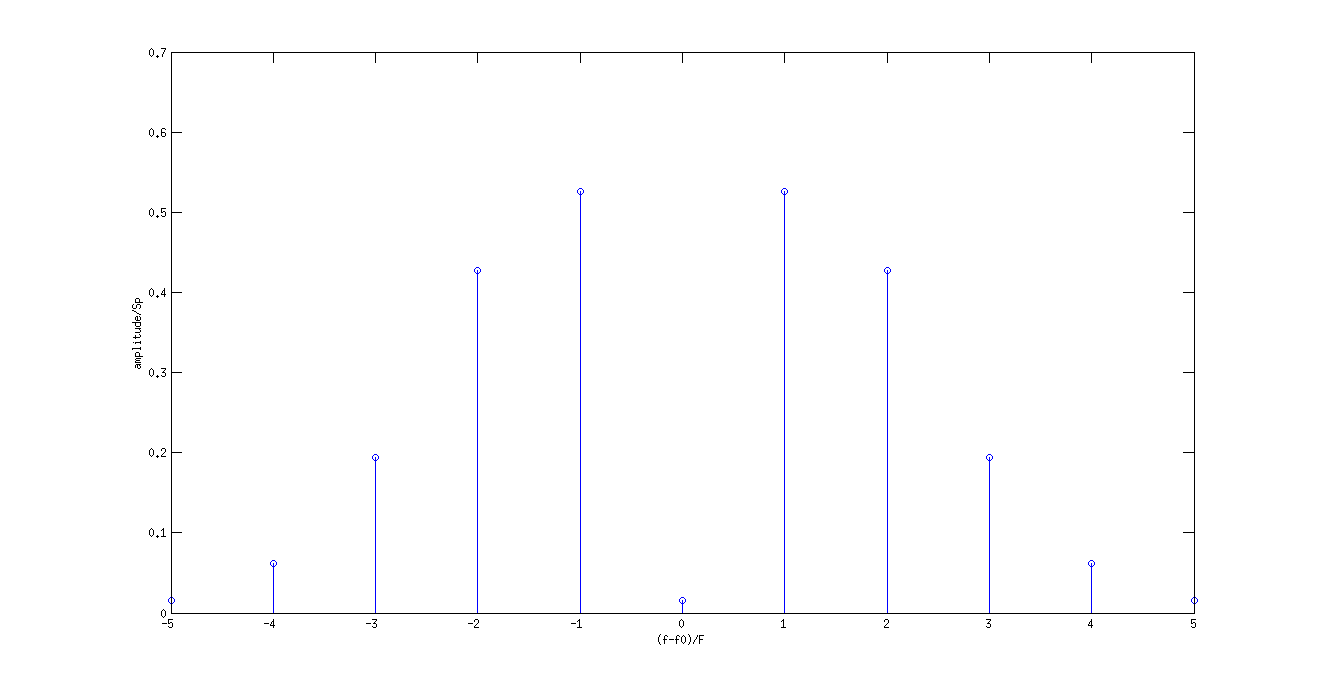
\includegraphics[width=\textwidth]{beta2375.png}
\caption{Spectre de $s(t)$ dans le cas $\beta = 2.375$}
\end{figure}

\item On considère le cas $\beta = 5$.

\begin{figure}[h!]
\centering
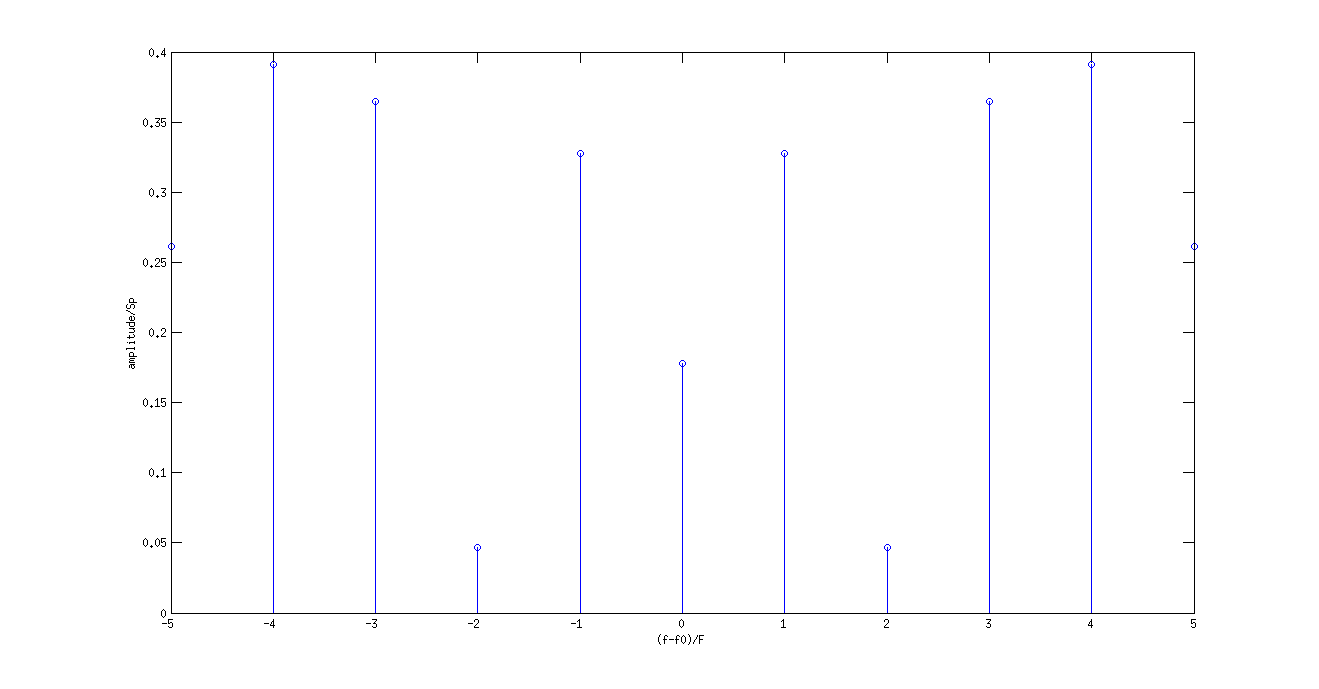
\includegraphics[width=\textwidth]{beta5.png}
\caption{Spectre de $s(t)$ dans le cas $\beta = 5$}
\end{figure}

\begin{center}
\begin{tabular}{|c|c|c|}
\hline
$\beta$ & $F$ & $B_u$ \\
\hline
5 & 2 kHz & 24 kHz \\ 
\hline
10 & 1 kHz & 22 kHz \\
\hline
15 & 0.67 kHz & 21.34 kHz \\
\hline
\end{tabular}
\end{center}

\item La modulation de fréquence est plus difficile à mettre en place que la modulation en amplitude. De plus, ce n'est pas une transformation linéaire, la bande de base n'est pas seulement transposée, et le spectre du signal modulé est plus large que pour une modulation AM. Cependant, la modulation FM réduit l'effet du bruit (notamment bruit additif dû à la transmission) par rapport à la modulation AM.

\item Si l'onde porteuse est un carré d'amplitude 5V et de valeur moyenne 2,5V, alors son spectre n'est plus une raie à $f_0$ mais un ensemble de raies à $f_0,3f_0...(2n+1)f_0$ avec des amplitudes en $\frac{1}{n}$. 

On pourrait penser que le spectre du signal modulé est beaucoup plus large et comporte beaucoup plus de raies.

Cependant, la seconde raie la plus importante a une amplitude 3 fois plus petite que celle à $f_0$. En terme d'énergie, elle compte donc pour environ 10 fois moins que la première. Cela signifie qu'on peut presque la négliger, et que l'on doit retrouver un spectre similaire à celui d'une onde sinusoïdal.
\end{itemize}

\subsection{Exemple de réalisation d'un modulateur de fréquence}

Notre signal modulant est un signal dont l'amplitude est variable. On cherche un circuit permettant de transposer des variations de tension en variations de fréquence. On utilise donc un oscillateur contrôlé en tension (VCO) réalisé dans un TP précédent. On choisit un VCO dont la plage de linéarité permet de générer une fréquence $f_0\pm \Delta f$ i.e. une fréquence appartenant à [50kHz,60kHz].

\section{Démodulation par boucle à verrouillage de phase}

\subsection{Étude des éléments de la PLL}

\subsubsection{Le VCO de la PLL}

On souhaite démoduler un signal dont la porteuse est à 60kHz. Il faut donc que le VCO ait une fréquence centrale d'oscillation de 60kHz, avec une plage de linéarité suffisante pour que la PLL reste accrochée, pour toute fréquence de [50kHz,60kHz].\\

On impose $R_2 = 10k\Omega$. Les abaques fournis dans la datasheet du 4046B nous permettent de choisir, avec $f_{min}=24kHz \et f_{max}=96kHz$,  \[C_1=3.3 \nano\farad \et \frac{R_2}{R_1}=4\]
donc
\[C_1=3.3 \nano\farad \et R_1 = 2.2\kilo\ohm\]

\subsubsection{Le comparateur de phase}

La caractéristique d'un comparateur de phase est une droite. Pour celui utilisé, on a sa caractéristique dans la datasheet et pour $V_{DD}=5 \volt$, la pente $K_1 =  2,8.10^{-2} \volt\per\degree$.

\begin{figure}[h!]
\centering
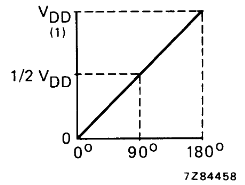
\includegraphics[scale=0.8]{caracXOR.png}
\caption{Caractéristique du comparateur de phase}
\end{figure}

Pour éviter que le comparateur de phase ne se verrouille sur fréquence harmonique non présente dans le signal, on utilise un condensateur en entrée du circuit pour filtrer les fréquences non utiles.


\subsubsection{Le filtre}

\begin{figure}[h!]
\centering
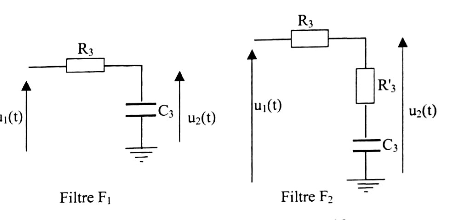
\includegraphics[scale=0.5]{filtresPB.png}
\caption{Filtres passe-bas}
\end{figure}

Pour le filtre $F_1$ :
\[F_1(p) = \frac{\frac{1}{C_3p}}{R_3+\frac{1}{C_3p}} = \frac{1}{1+\tau p} \avec \tau = R_3C_3\]

Pour le filtre $F_2$ :
\[F_2(p) = \frac{R'_3+\frac{1}{C_3p}}{R_3+R'_3+\frac{1}{C_3p}} = \frac{1+\tau_1 p}{1+\tau_2 p} \avec \tau_1 = R'_3C_3 \et \tau_2 = (R_3+R'_3)C_3\]


\subsection{Choix des éléments du filtre pour réaliser un démodulateur de fréquence}

\subsubsection{Mise en équation}
Le schéma-bloc d'une boucle à verrouillage de phase est :

\begin{figure}[h!]
\centering
\begin{tikzpicture}
\sbEntree{E}

\sbBloc[4]{comp}{Comparateur de phase}{E}           
\sbRelier[$v_e(t)$]{E}{comp}

\sbBloc[4]{pb}{Filtre passe-bas}{comp}
\sbRelier[$v_1(t)$]{comp}{pb}

\sbBloc[4]{sys}{VCO}{pb}
\sbRelier[$v_2(t)$]{pb}{sys}

\sbSortie[4]{S}{sys}
\sbRelier[$v_s(t)$]{sys}{S}

\sbRenvoi{sys-S}{comp}{}

\end{tikzpicture}
\caption{Schéma de principe d'une PLL}
\end{figure}

Lorsque la boucle est verrouillée, alors la fréquence  de $v_s(t)$ est la même que celle de $v_e(t)$. Par conséquent, si la fréquence de $v_e(t)$ est contrôlée par un signal modulant, alors on retrouve en entrée du VCO, qui contrôle la fréquence de $v_s(t)$, l'image du signal modulant.

\begin{figure}[h!]
\centering
\begin{tikzpicture}
\sbEntree{E}

\sbBloc[4]{int}{$\frac{2\pi}{p}$}{E}
\sbRelier[$F_e(p)$]{E}{int}

\sbComp[4]{comp}{int}                
\sbRelier[$\Phi_e(p)$]{int}{comp}

\sbBloc[4]{phcomp}{$K_1$}{comp}  
\sbRelier{comp}{phcomp}

\sbBloc[6]{H}{$F(p)$}{phcomp}      
\sbRelier[$U_1(p)$]{phcomp}{H}

\sbSortie[4]{S}{sys}
\sbRelier[$U_2(p)$]{H}{S}       

\sbDecaleNoeudy[4]{S}{R}
\sbBlocr[12]{intr}{$K_2\frac{2\pi}{p}$}{R}
\sbRelieryx{sys-S}{intr}
\sbRelierxy[$\Phi_s(p)$]{intr}{comp}

\end{tikzpicture}
\caption{Schéma bloc de la PLL}
\end{figure}
On a donc :
\[ U_2(p) = F(p)K_1\frac{2\pi}{p}(F_e(p) - K_2U_2(p)) \]
La fonction de transfert en boucle fermée de ce schéma-bloc est :

\[ \frac{U_2(p)}{F_e(p)} =  \frac{2\pi K_1F(p)}{p+2\pi K_1K_2 F(p)} \]

En basse fréquence, $F(p)$ a un gain constant, donc on a la relation directe $U_2(p) = \frac{F_e(p)}{K_2}$ et $F_e(p)$ est proportionnelle au signal modulant.\\

Il faut que la bande passante $f^{BF}$ soit suffisante pour laisser passer la fréquence maximale du signal modulant, mais qu'elle coupe les fréquences de la porteuse et celles introduites par la modulation pour assurer une démodulation correcte.

\subsection{Étude dans le cas du filtre $F_1(p)$}
Avec $F_1(p)=\frac{1}{1+\tau p} \avec \tau = R_3C_3$, on obtient :
\[ \frac{U_2(p)}{F_e(p)} = \frac{1}{K_2}\frac{1}{\frac{\tau}{2\pi K_1 K_2}p^2 + \frac{1}{2\pi K_1 K_2}p +1}\]

On en déduit donc $f_{BF} = \sqrt{\frac{K_1 K_2}{2\pi \tau}}$ et $\xi = \frac{1}{2\sqrt{2\pi K_1 K_2 \tau}}$. 

Ces deux paramètres ne peuvent donc pas être réglés indépendamment. \\

En imposant $f_{BF}$, on a donc :
\[ \tau = \frac{K_1 K_2}{2\pi f_{BF}^2} \et \xi = \frac{f_{BF}}{2K_1K_2} \]

\subsection{Étude dans le cas du filtre $F_2(p)$}
Avec $F_2(p) = \frac{1+\tau_1 p}{1+\tau_2 p} \avec \tau_1 = R'_3C_3 \et \tau_2 = (R_3+R'_3)C_3$, on a 
\[ \frac{U_2(p)}{F_e(p)} = \frac{1}{K_2} \frac{1+\tau_1 p}{\frac{\tau_2}{2\pi K_1K_2}p^2 + (\tau_1+\frac{1}{2\pi K_1K_2})p+1}\]

On a donc 
$f_{BF} = \sqrt{\frac{K_1 K_2}{2\pi \tau_2}}$ et $\xi = \frac{1+2\pi K_1 K_2 \tau_1}{2\sqrt{2\pi K_1 K_2 \tau_2}}$.

On peut donc régler $f_{BF}$ en agissant uniquement sur $\tau_2$, puis régler $\xi$ en agissant sur $\tau_1$.\\

En imposant $f_{BF}$ et $\xi$, pn a alors :

\[ \tau_2 = \frac{K_1K_2}{2\pi f_{BF}^2} \et \tau_1 = \frac{2\xi K_1 K_2 - 1}{2\pi K_1 K_2} \]

\newpage
\begin{center}
\begin{Large}
B. Manipulation
\end{Large}
\end{center}
\setcounter{section}{0}

\section{Étude des propriétés d'une onde modulée en fréquence}

On génère le signal modulée en fréquence avec le GBF : on choisit un signal porteur sinusoïdal de fréquence 60 kHz, d'excursion de fréquence 10kHz. On fait ensuite varier la valeur de $F_M=F$, c'est-à-dire la largeur de la bande de base.

\begin{itemize}\setlength{\itemsep}{10mm}
\item  On cherche les valeurs de la fréquence de modulation $F$ (i.e. de $\beta$) qui annulent la composante à la fréquence centrale des spectres.\\

\begin{center}
\begin{tabular}{|c|c|c|}
\hline 
$\beta$ tel que $J_0(\beta)=0$ & F (théorique) & F (relevée)  \\ 
\hline 
2.375 & 4.21 kHz & 4,16 kHz \\ 
\hline 
5.625 & 1.78 kHz & 1,81 kHz \\ 
\hline 
8.875 & 1.13 kHz & 1,15 kHz \\ 
\hline 
\end{tabular} 
\end{center}

\begin{figure}[h!]
\centering
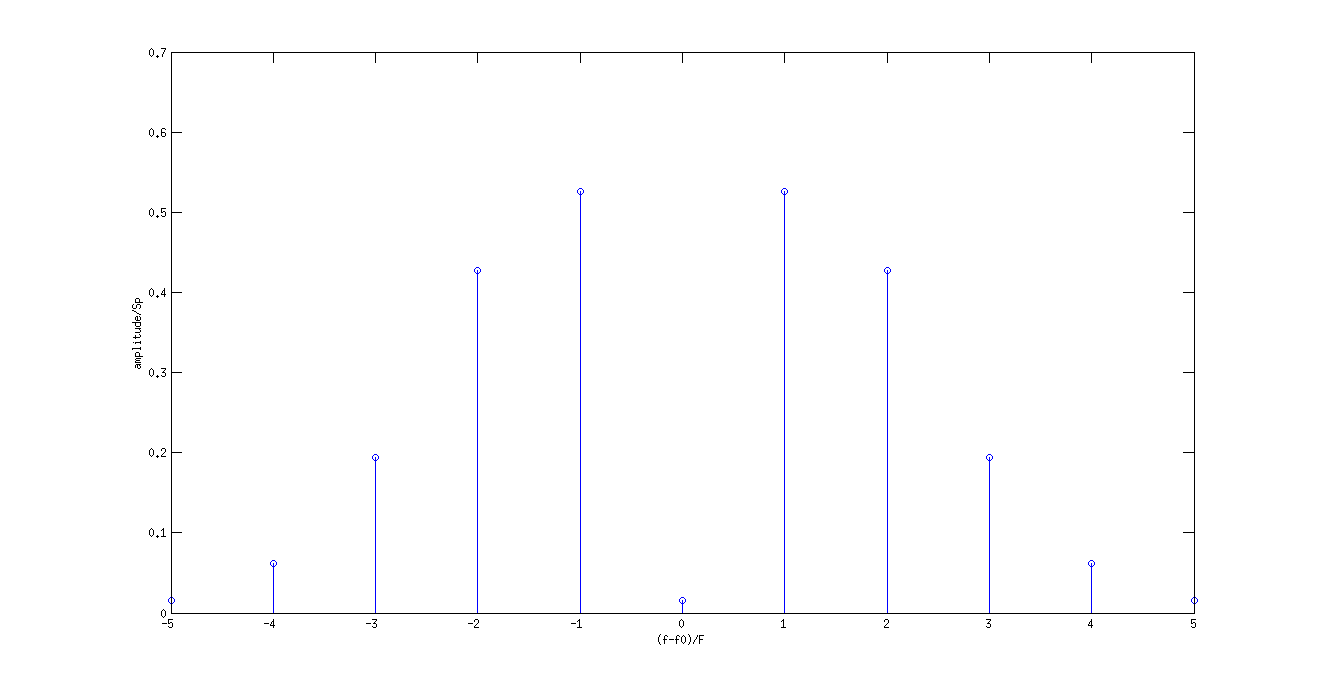
\includegraphics[width=0.6\textwidth]{beta2375.png}
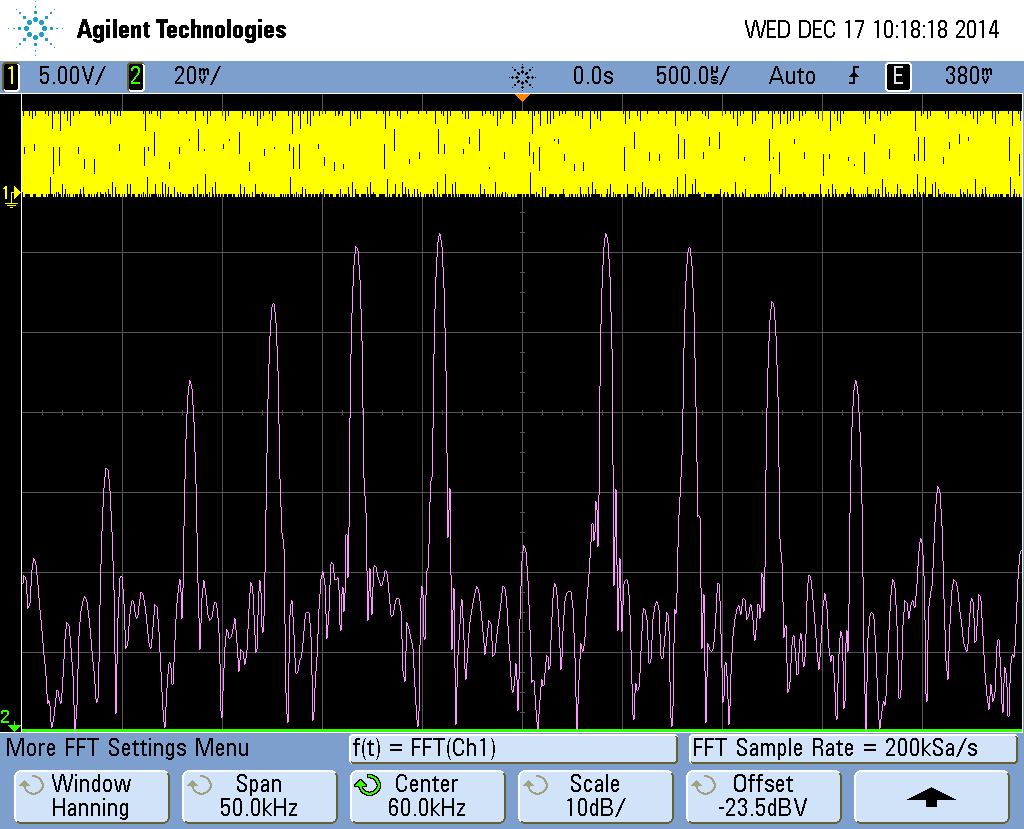
\includegraphics[width=0.6\textwidth]{bessel03.png}
\caption{Spectres théorique et relevé, pour $\beta=2.375$, et pour une fréquence F théorique de 4,21 kHz et relevée de 4,16 kHz}
\end{figure}

Les observations sont en accord avec la préparation.

\item On mesure ensuite la largeur de spectre du signal modulé pour les valeurs de $\beta$ égales à 5,10 puis 15. Comme on ne peut pas facilement déterminer la bande pour laquelle la puissance du signal est de 98 \%, on place les curseurs sur la bande théorique déterminée et on détermine l'importance des raies rejetées par rapport aux autres.\\

\newpage
\begin{figure}[h!]
\centering
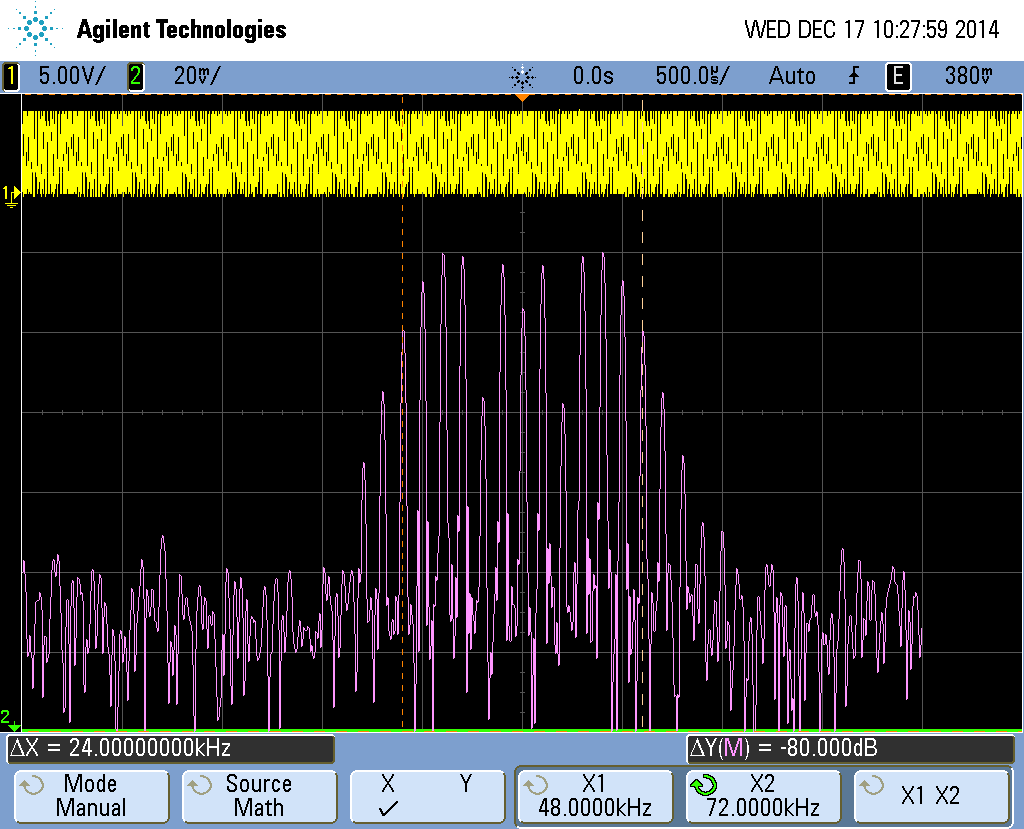
\includegraphics[width=0.6\textwidth]{carson5.png}
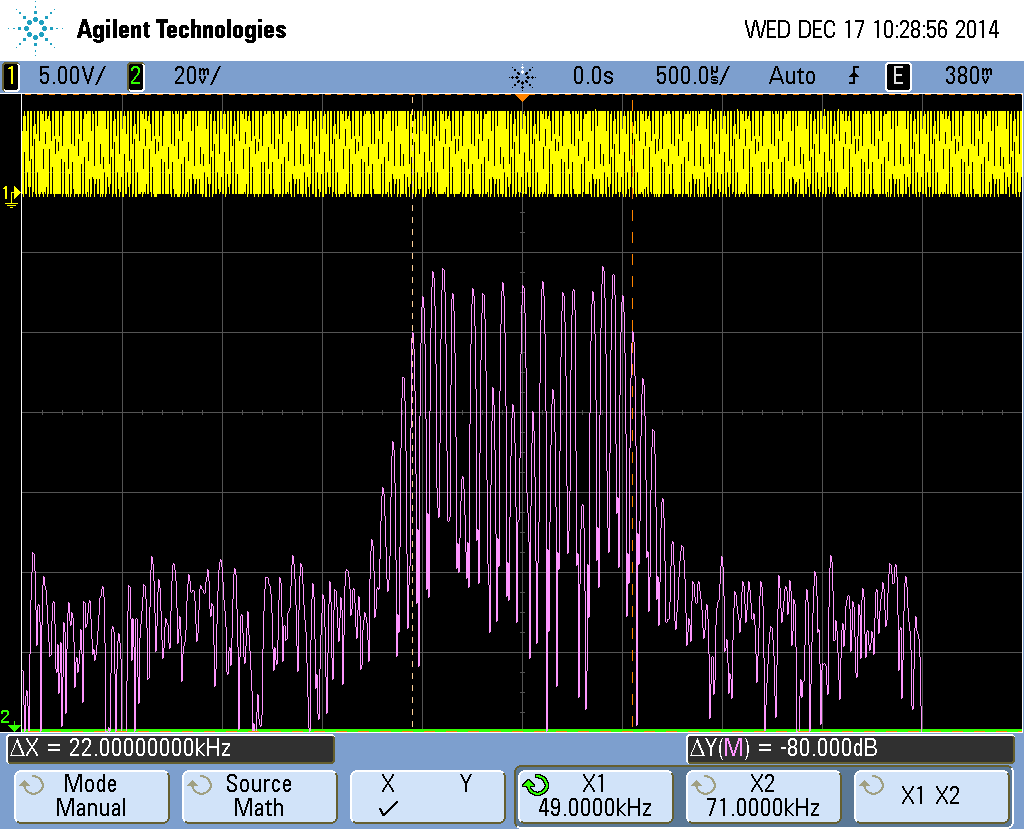
\includegraphics[width=0.6\textwidth]{carson10.png}
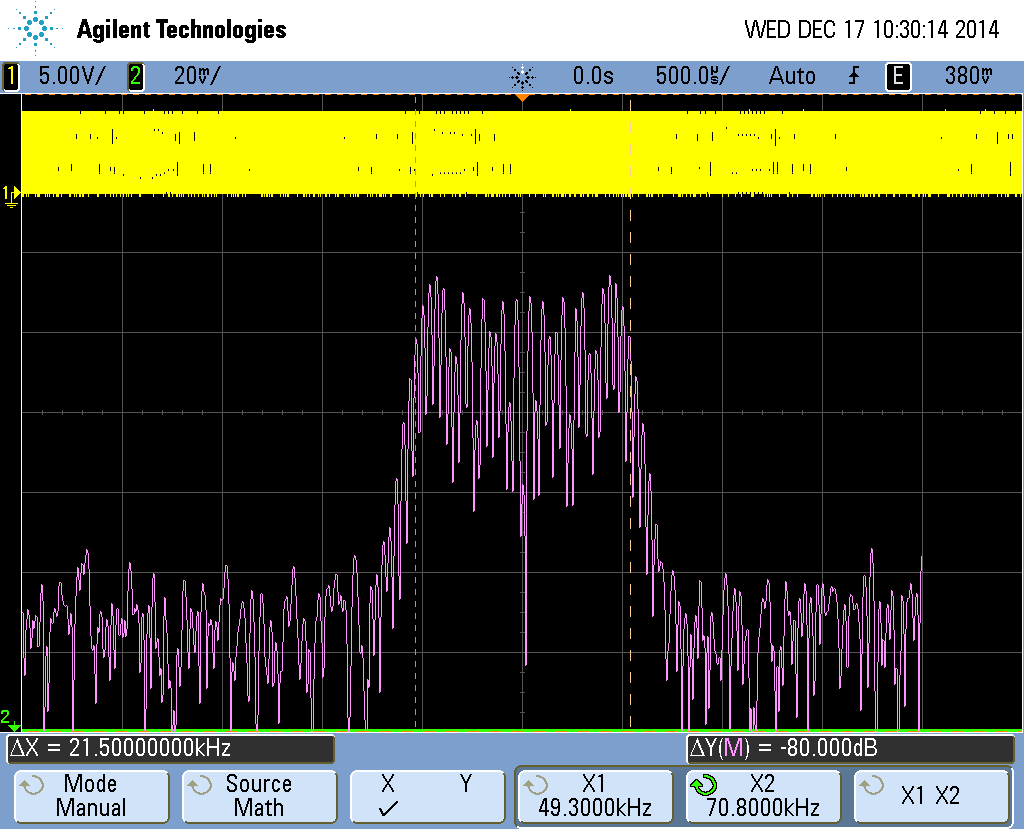
\includegraphics[width=0.6\textwidth]{carson15.png}
\caption{Spectres et bandes de Carson pour $\beta$ = 5,10 puis 15}
\end{figure}

\newpage Dans le cas $\beta=5$, où la bande théorique de Carson est de 24 kHz, on a le spectre suivant :
\begin{figure}[h!]
\centering
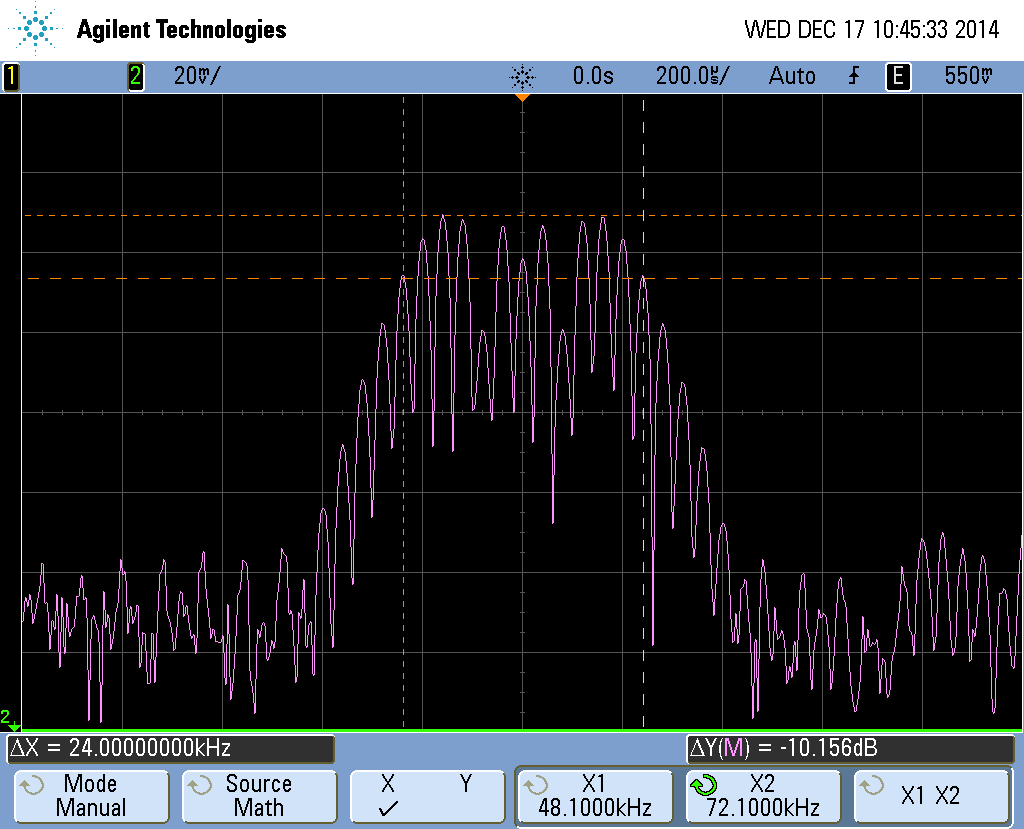
\includegraphics[width=0.6\textwidth]{carson5dB.png}
\caption{Spectre et bande de Carson pour $\beta$ = 5}
\end{figure}

La première raie rejetée a un rapport d'amplitude de -10 dB par rapport à la plus énergétique, ce qui signifie qu'il y a un rapport 10 entre les deux amplitudes, donc un rapport 100 en puissance. Toutes les raies rejetées sont au moins 100 fois moins énergétiques que les plus importantes : l'observation est bien en accord avec la règle de Carson.

\item On considère un signal porteur carré d'amplitude 0-5V, de fréquence $f_0=2kHz$, $\beta = 5$
\begin{figure}[h!]
\centering
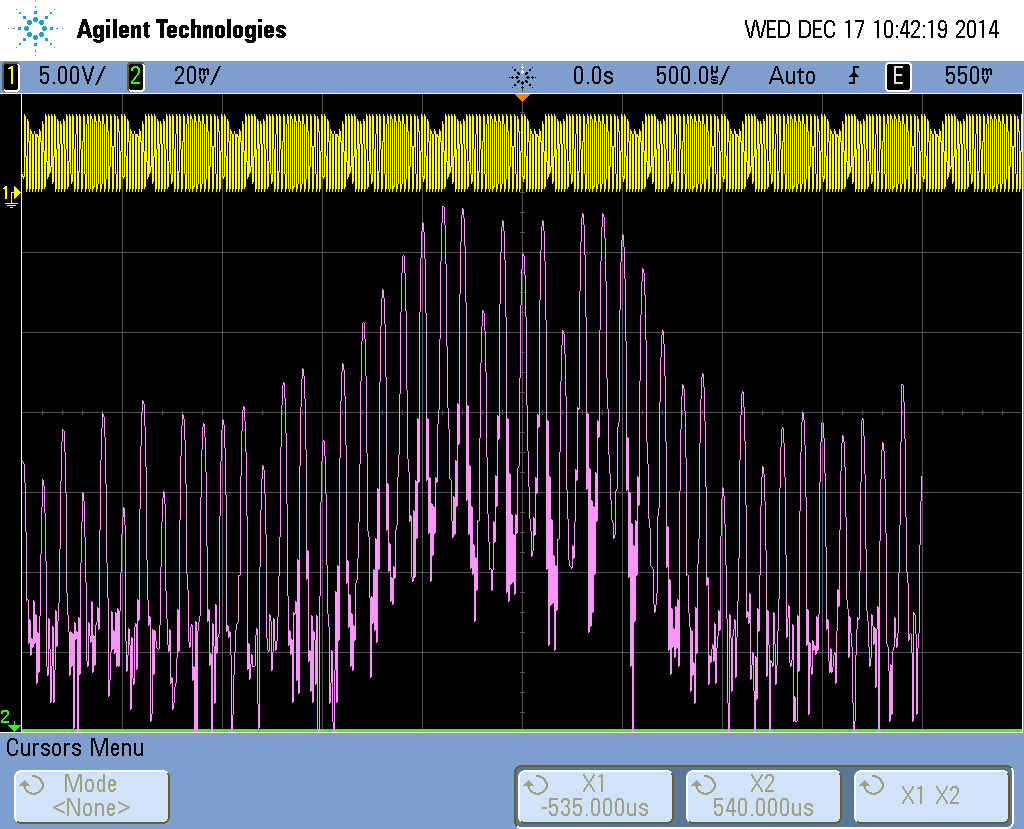
\includegraphics[width=0.6\textwidth]{porteusecarree.png}
\caption{Spectre du signal modulé dans le cas d'une porteuse carrée}
\end{figure}

Dans le cas d'une porteuse carrée, on observe un spectre plus large, mais similaire au spectre obtenu pour une porteuse sinusoïdale (Figure 6). En effet, les pics introduits par le caractère carré de la porteuse ont un rapport de plus de 26 dB avec les raies les plus importantes, c'est-à-dire un rapport d'amplitude de plus de 400. Ces raies sont donc vraiment négligeables, et la bande de Carson n'est pas modifiée dans le cas d'une porteuse carrée.
\end{itemize}

\section{Étude de l'émetteur}

On trace la caractéristique $f(E)$ de l'oscillateur contrôlé en tension (VCO), pour $E$ allant de 0 à 4V.

\begin{figure}[h!]
\centering
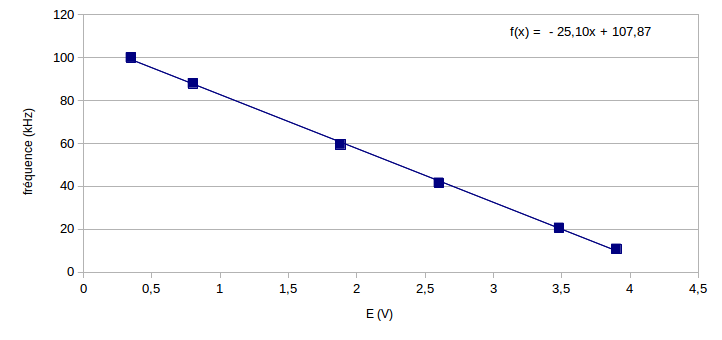
\includegraphics[width=\textwidth]{f(E).png}
\caption{Caractéristique $f(E)$ du VCO pour $E$ allant de 0 à 4V}
\end{figure}

La caractéristique est une droite d'équation : $f(E) = -25.10E+107.87$ (en kHz). Ainsi, pour avoir une fréquence porteuse de 60 kHz, il faut $E = 1.9V$. Pour obtenir une excursion de fréquence de 10 kHz, il faut avoir une amplitude de $\Delta E = 0,4V$.\\

Avec le GBF, on génère donc un signal sinusoïdal de fréquence $F=2kHz$, d'amplitude peak-to-peak 0,8V et de valeur moyenne 1.83V. On obtient en sortie du VCO le signal modulé dont le spectre est donné ci-dessous :

\begin{figure}[h!]
\centering
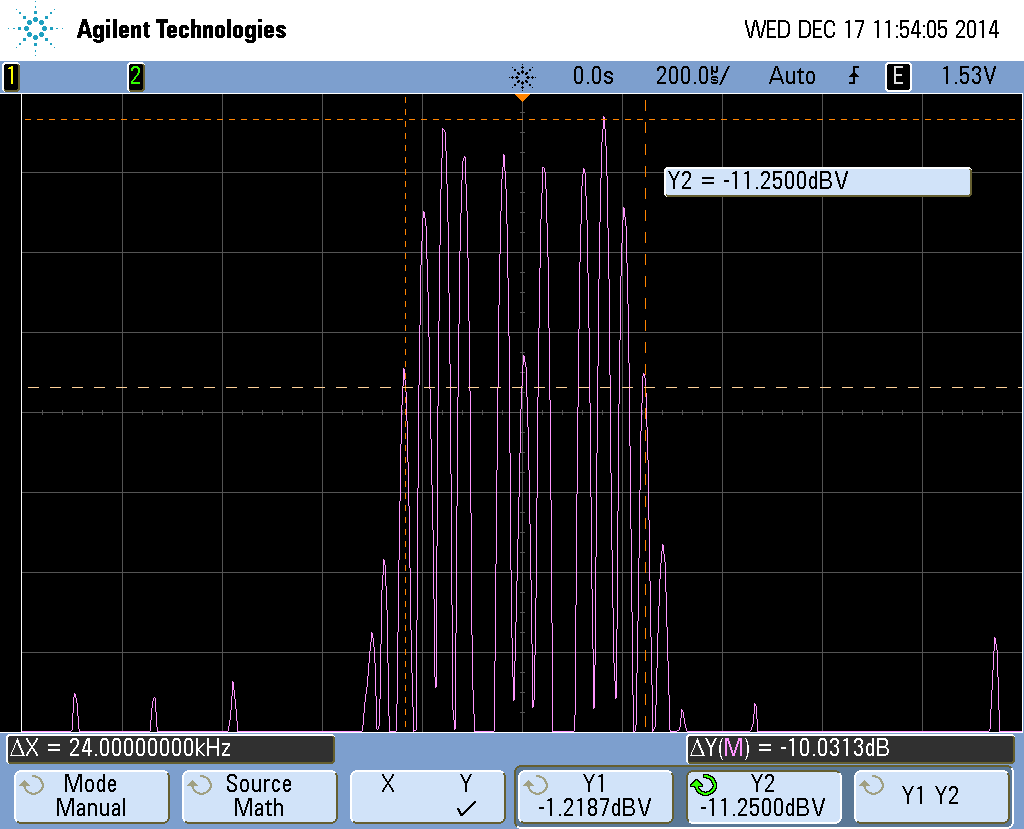
\includegraphics[width=0.6\textwidth]{modVCO.png}
\caption{Spectre du signal modulé en sortie du VCO}
\end{figure}

Le spectre du signal est centré sur $f_0 = 60kHz$. La bande de Carson est de 24kHz, ce qui était attendu pour un signal modulé de porteuse 60kHz, d'excursion 10kHz et ayant une modulante de fréquence 2kHz.

\section{Étude du récepteur}

\subsection{Étude de la PLL 4046B}

\subsubsection{Caractérisation du VCO de la PLL}
On prend $R_2 = 10k\Omega$, $R_1 = 2.2k\Omega$. Si on prend $C_1 = 3.3 nF$ pour obtenir une fréquence d'oscillation de $f_0 = 60 kHz$ à $E=2.5V$, alors on se trouve en limite de la plage de linéarité du VCO. 

On préfère changer $C_1$ pour être vraiment dans la plage de linéarité. On prend $C_1=4,7nF$.\\

On trace la caractéristique $f(E)$ du VCO de la PLL :

\begin{figure}[h!]
\centering
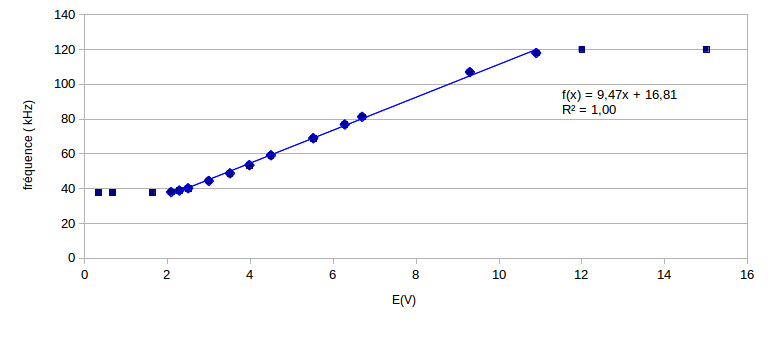
\includegraphics[width=\textwidth]{f(E)2.png}
\caption{Spectre du signal modulé en sortie du VCO}
\end{figure}

La plage de linéarité est de 38kHz à 118 kHz, pour une tension de polarisation comprise entre 2 et 11 V ($V_{DD} = 15V$). Le gain $K_2$ est de 9.42 kHz / V.

\subsubsection{Comportement de la PLL}
On place $R_3 = 12 k\Omega$ et $C_3 = 1nF$, soit une bande passante de $13 kHz$. 

La plage de capture est [53kHz;120kHz]. La plage de verrouillage est [34kHz;125kHz].

Avec des fréquences comprises entre 50 kHz et 70 kHz, la boucle peut se verrouiller sur les différentes fréquences du signal modulant.

\newpage
\subsection{Démodulation par boucle à verrouillage de phase}

\subsubsection{Cas du filtre passe-bas de fonction de transfert $F_1(p)$}

On utilise le premier VCO pour générer un signal modulé. On applique pour cela en entrée du VCO un signal carré d'amplitude 0.4V et de valeur moyenne 1.83V. La fréquence est $F=2 kHz$.\\

On obtient en sortie de PLL le signal suivant :

\begin{figure}[h!]
\centering
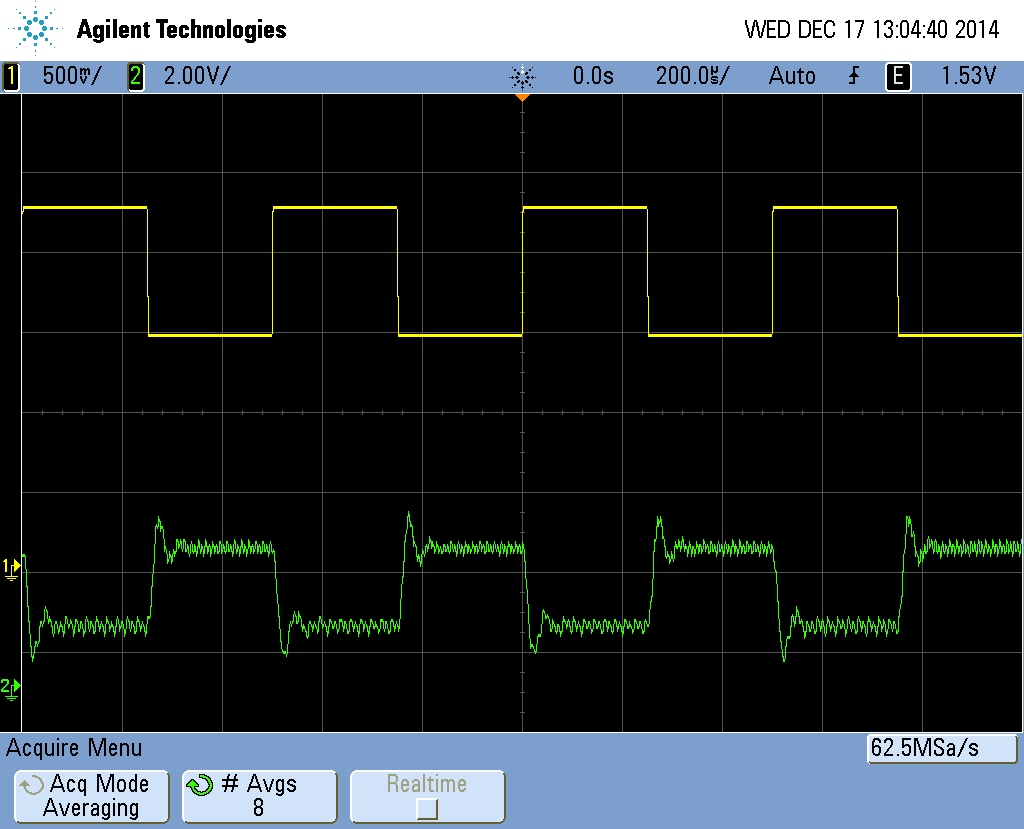
\includegraphics[width=\textwidth]{moddemod.png}
\caption{Signal modulant et signal démodulé}
\end{figure}

On observe que le signal démodulé correspond à la réponse indicielle d'un système du second ordre. La pseudo pulsation du système est de l'ordre de $78.10^{3}$rad/s, et le premier dépassement d'environ 40\%.

\newpage
\subsubsection{Cas du filtre passe-bas de fonction de transfert $F_2(p)$}

On utilise le deuxième filtre passe-bas afin de pouvoir régler indépendamment $\omega_0$ et $\xi$. En utilisant $R_3=R_3'$, on obtient la réponse suivante :

\begin{figure}[h!]
\centering
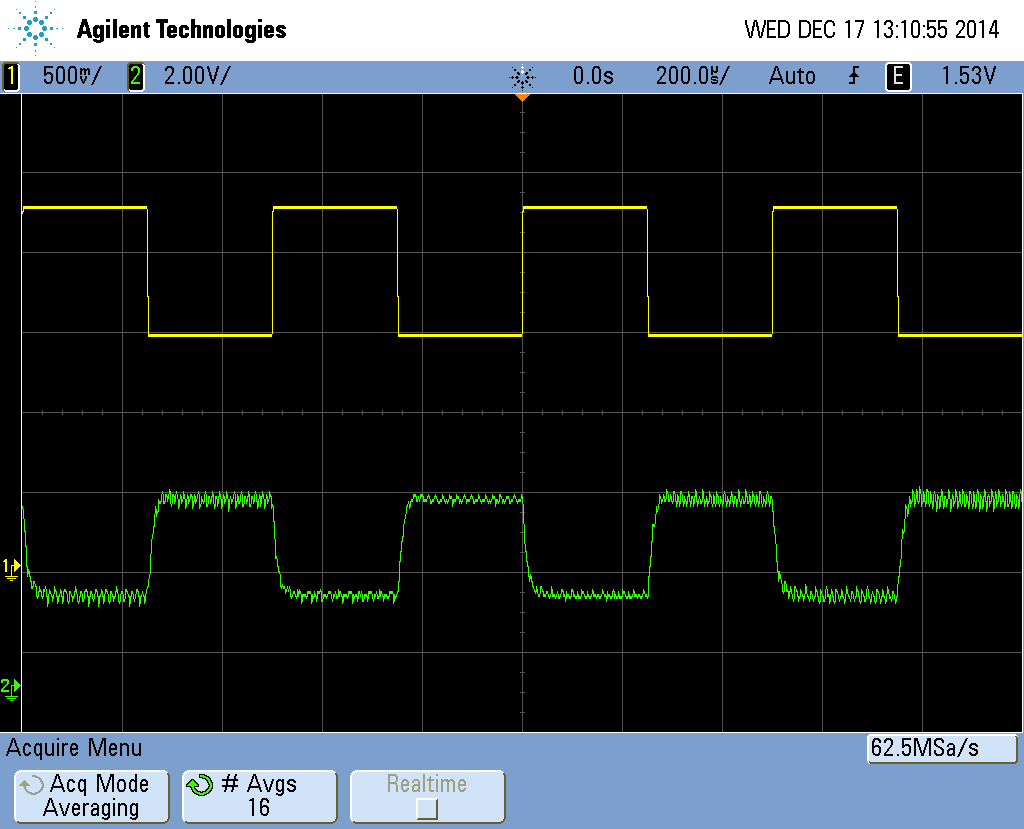
\includegraphics[width=\textwidth]{moddemod2R.png}
\caption{Signal modulant et signal démodulé}
\end{figure}

Les oscillations dues au filtre d'ordre 2 ont été amorties.

\section*{Conclusion}

Dans ce TP, nous avons mis en oeuvre une technique de modulation et de démodulation de fréquence. Nous avons étudié l'importance du choix des plages de fonctionnement des VCO, aussi bien lors de l'émission que lors de la boucle à verrouillage de phase servant à la démodulation.



\end{document}
